\documentclass[12pt]{article}
\usepackage[left=1in,top=1in,right=1in,bottom=1in]{geometry}
\usepackage[font=footnotesize]{caption}
\usepackage{parskip}
\usepackage{times}
\usepackage{graphicx}
\usepackage{mathtools}
\usepackage{gensymb}
\usepackage{placeins}

\setlength{\parskip}{\baselineskip}

\newcommand{\bfvec}[1]{\overline{\mathbf{#1}}}
\newcommand{\spaces}{\phantom{\qquad}}
\newcommand{\under}{\underline{\phantom{\enspace}}}
\newcommand{\diff}{\frac{\mathrm{d}}{\mathrm{d}t}}
\newcommand{\dif}{\mathrm{d}}

\begin{document}

	\subsubsection*{Simulation}
	
	Source: http://www.myphysicslab.com/runge\_kutta.html \\
	Source: http://en.wikipedia.org/wiki/List\_of\_Runge\%E2\%80\%93Kutta\_methods
	
	Simulation usually involves integration, for example for an object in free fall. In that case, we would have the variables $s$, $v$, $a$, and $t$. The most basic way of implementing integration in a computer program is Euler's method, which is basically choosing a very small time interval $h$ and then incrementing each variable by their derivative multiplied by $h$.

	Say we have a ``vector'' $\bfvec{X} = (s, v, a)$, where $\bfvec{X}$ is a ``vector'' containing all of the variables in the system. Next, let $\bfvec{X'} = (v, a, 0)$, where $\bfvec{X'}$ is a ``vector'' containing the derivative of every variable in the system.

	Suppose that $\bfvec{X}_n$ is the value of the variables at time $t$ and that $\bfvec{X}_{n+1}$ is the value of the variables at time $t+h$. Then Euler's method is basically
			$$\bfvec{X}_{n+1} = \bfvec{X}_n + h\,\bfvec{X'}_n$$			
	This can be generalized for any system of variables. Suppose that there are $m$ variables $x_1$,~$x_2$,~...,~$x_m$, each of which vary over time. In the free fall example, $x_1$ would be position and $x_2$ would be velocity. Suppose there are $m$ differential equations for these $m$ variables
			$$x_1' = f_1(t_n, x_1,x_2,...,x_m)$$
			$$x_2' = f_2(t_n, x_1,x_2,...,x_m)$$
			$$...$$
			$$x_m' = f_m(t_n, x_1,x_2,...,x_m)$$
	Note that each function takes every other variable as an argument even though we don't necessarily need to use every variable. For example, in the free fall example, the derivative of acceleration would just be 0, which is not dependent on either position or velocity. But for ease of programming, we send all of those variables in as arguments anyway. Rather than cherry-picking which variable this derivative function will require, it's a lot easier to just send all of them and let the function decide which ones to use. 
	
	These equations can be summarized in vector form as
			$$\bfvec{X'} = \bfvec{f}(t_n, \bfvec{X})$$
	where $\bfvec{X} = (x_1,x_2,...,x_m)$ and $\bfvec{f}=(f_1,f_2,...,f_m)$ in a loose ``vector of functions'' sort of concept. So say we label our time states $\bfvec{X}_n$, $\bfvec{X}_{n+1}$, which are separated by a time interval of length h. Then
			$$\bfvec{X}_n = (x_{1,n}, x_{2,n}, ..., x_{m,n})$$
			$$\bfvec{X}_{n+1} = (x_{1,n+1}, x_{2,n+1}, ..., x_{m,n+1})$$
	So if we have the state of the simulation at time $t_n$ as $\bfvec{X}_n$, we want to compute the state a short time $h$ later and put the results into $\bfvec{X}_{n+1}$. And then do the same for $\bfvec{X}_{n+1}$ and $\bfvec{X}_{n+2}$, and keep going until a stopping condition is reached. This is either the user pressing the exit button on the top right corner of the screen, or some sort of calculated limit that the programmer puts in.

	\subsubsection*{Integration Methods}
	
	We know that Euler's method is
			$$\bfvec{X}_{n+1} = \bfvec{X}_n + h\,\bfvec{X'}_n$$
	but we would need a very small time step to achieve any sort of accuracy, and that is computationally expensive. There is a family of integration methods called Runge-Kutta methods, and Euler's method is the simplest of all of them. Euler's method is denoted RK1. Higher order RK methods use things like midpoint rule or Simpson's rule to achieve higher accuracy for the same time interval. For example, RK4, or ``\textit{the} Runge-Kutta method'', does the following:
			$$\bfvec{a}_n = \bfvec{f}(t_n, \bfvec{X}_n)$$
			$$\bfvec{b}_n = \bfvec{f}(t_n + \frac{h}{2},\bfvec{X}_n + \frac{h}{2}\ \bfvec{a}_n)$$
			$$\bfvec{c}_n = \bfvec{f}(t_n + \frac{h}{2},\bfvec{X}_n + \frac{h}{2}\ \bfvec{b}_n)$$
			$$\bfvec{d}_n = \bfvec{f}(t_n + h, \bfvec{X}_n + h\ \bfvec{c}_n)$$
			$$\bfvec{X}_{n+1} = \bfvec{X}_n + \frac{h}{6}\ (\bfvec{a}_n + 2\ \bfvec{b}_n + 2\ \bfvec{c}_n + \bfvec{d}_n)$$			
	A general Runge-Kutta method can be specified using a Butcher tableau, which is of the form	
			\[\begin{array}{c|cccc}
				c_1    & a_{11} & a_{12}& \dots & a_{1s}\\
				c_2    & a_{21} & a_{22}& \dots & a_{2s}\\
				\vdots & \vdots & \vdots& \ddots& \vdots\\
				c_s    & a_{s1} & a_{s2}& \dots & a_{ss} \\
				\hline
       			& b_1    & b_2   & \dots & b_s\\
			\end{array}\]
	The Runge-Kutta method for a particular Butcher tableau is defined as follows:
			$$\bfvec{X}_{n+1} = \bfvec{X}_n + h \sum_{i=1}^s b_i k_i$$
			$$k_i = \bfvec{f}\left(t_n + c_i h, \bfvec{X}_n + h \sum_{j = 1}^{s} a_{ij} k_j\right)$$

	In the solenoid simulator, $t$ is not time but rather some parameter, but the general concept is the same. The Butcher tableau for the RK1 method that we used is:
			\[\begin{array}{c|c}
				0 & 0 \\
				\hline
  				  & 1 \\
			\end{array}\]			
	The Butcher tableau for the RK2 method that we used is:	
			\[\begin{array}{c|cc}
				0   & 0   & 0  \\
				1/2 & 1/2 & 0  \\
				\hline
    				& 0   & 1  \\
			\end{array}\]			
	The Butcher tableau for the RK4 method that we used is:
			\[\begin{array}{c|cccc}
				0   & 0   & 0   & 0   & 0\\
				1/2 & 1/2 & 0   & 0   & 0\\
				1/2 & 0   & 1/2 & 0   & 0\\
				1   & 0   & 0   & 1   & 0\\
				\hline
    				& 1/6 & 1/3 & 1/3 & 1/6\\
			\end{array}\]
	The Butcher tableau for the RK5 method that we used is:
			\[\begin{array}{c|cccccc}
				0     & 0         & 0          & 0           & 0          & 0        & 0\\
				1/4   & 1/4       & 0          & 0           & 0          & 0        & 0\\
				3/8   & 3/32      & 9/32       & 0           & 0          & 0        & 0\\
				12/13 & 1932/2197 & -7200/2197 & 7296/2197   & 0          & 0        & 0\\
				1     & 439/216   & -8         & 3680/513    & -845/4104  & 0        & 0\\
				1/2   & -8/27     & 2          & -3544/2565  & 1859/4104  & -11/40   & 0\\
				\hline
    		    0     & 16/135    & 0          & 6656/12825  & 28561/56430&-9/50     & 2/55\\
			\end{array}\]
	The RK1 is a first order method, called the ``Forward Euler''. It lacks stability, which means any error introduced accumulates in a positive feedback loop. It also has significant accuracy limits, so it is not an ideal integration method if any accuracy is desired.
	
	The RK2 is a second order method, called the ``Explicit midpoint method''.	The RK4 is a fourth order method; the ``original'' Runge-Kutta method. The RK5 is a fifth order method; the ``Runge-Kutta-Fehlberg method''.
	
	All of the RK methods of order greater than 1 exhibit elements of numerical stability, which is good because then any errors introduced in the numerical integration tend to be damped out. The effect of a higher-order RK method is basically to provide the same level of accuracy for a larger time interval, which reduces computational cost. 
	
	\subsubsection*{Magnetism}
	
	Okay, about that $t$ not being time business. See, we want to know the magnetic field of a particular system of wires and current in 3-space in one particular moment in time. Obviously in real life, this field would then induce emfs in the wires and then change the state of the wires which would then change the magnetic and electric fields and ugh that's too complicated. Our simulation is going to have solenoids floating in space not connected to a power source, so obviously it's not going to be accurate in that sense.
	
	We are only concerned with $\vec{B}$ at this instant in time. So remember, $t$ is not time. It is a parameter. This is useful because our wires are 1D functions in 3D, so the x,y,z coordinates can be computed as a function of this single parameter. ``Regrettably, the variable $t$ is often chosen to represent the parameter. One must remember that this has nothing to do with time!''(van Bemmel, 04 Sep 2014). In our case, it is rather fortunate that the parameter is $t$ because that means we don't have to change notation (lazy).
	
	First principles time. From Mr. van Bemmel's biotsavart primer, the law of Biot-Savart describes the differential magnetic field due to a current element by:	
			$$\dif \vec{B} = \frac{\mu_0}{4\pi} \, \frac{i\,\dif \vec{s} \times \hat{r}}{r^2}$$			
	Where: \\
		\spaces $\dif \vec{B}$ = the differential magnetic field at one specific reference point (T) \\
		\spaces $\mu_0 =$ the permeability constant (exactly 4$\pi \times 10^{-7}$ TmA$^{-1}$)\\		
		\spaces $i$ = the current in the current element (A) \\
		\spaces $\dif \vec{s}$ = the differential position on the current element (m) \\
		\spaces $\hat{r}$ = the unit position vector pointing from the current element to the reference point (m)\\
		\spaces $r$ = the magnitude of the distance between the current element and the reference point (m)
			
	To determine the $\vec{B}$ at a specific reference point, we sum all of these little $d\vec{B}$'s along the wire. Thus, the general algorithm is this: For each reference point, find the numerical integral of $d\vec{B}$ along each wire and sum the results of each wire to get the $\vec{b}$ at that point. We can sum the individual $\vec{B}$ caused by each wire because of the superposition principle: $\vec{B}$ is additive.
	
	To compute this integral, we need the following variables: \\
		\spaces 1. $\vec{P}$ - the position of the reference point (m)\\
		\spaces 2. $\vec{s}$ - the position on the wire (m)\\
		\spaces 3. $\vec{B}$ - the magnetic field at the reference point (T)
		
	We don't really need $\hat{r}$ since it can easily be computed from $\vec{P} - \vec{s}$. If we parameterize these variables with the parameter $t$, then
			$$\vec{P}_0 = (P_x, P_y, P_z)$$
			$$\vec{s}_0 = \text{get\under s}(t_i)$$
			$$\vec{B}_0 = (0, 0, 0)$$
	We can set $\vec{P}$ to whatever we want, and we begin $\vec{B}$ with the additive identity, the zero vector. We will denote the position on the wire with the function get\under s$(t_i)$ now, as this is dependent on the geometry of the wire. Here $t_i$ represents the value of $t$ that gives the start of the wire. We will get more into that later. Next, finding the derivatives with respect to t, we have:
			$$\diff \vec{P} = (0, 0, 0)$$
			$$\diff \vec{s} = \text{diff\under s}(t)$$
			$$\diff \vec{B} = \frac{\mu_0}{4\pi} \, \frac{i\,\diff \vec{s} \times \widehat{(\vec{P} - \vec{s})}}{|\vec{P} - \vec{s}|^2}$$	
	The derivative of $\vec{P}$ is zero because it is constant. Also, because the current and permeability constant are... well, constant for each wire, we can save a bit of computational time by factoring these constants out of the integral, and multiplying the $\vec{B}$ by the constant only after the integral is done. Thus, we compute
			$$\vec{B} = \sum \frac{\mu_0 \, i_k}{4\pi}\int\frac{\diff \vec{s} \times \widehat{(\vec{P} - \vec{s})}}{|\vec{P} - \vec{s}|^2} \, \dif t$$	
	Where $i_k$ is the current in the kth wire being integrated. We have almost everything we need for the Runge-Kutta algorithm to be implemented now. Let
			$$\bfvec{X} = (\vec{P},\vec{s},\vec{B})$$
			$$\bfvec{X'} = \left(\diff\vec{P},\diff\vec{s},\diff\vec{B}\right)$$
	Recall that a Runge-Kutta algorithm is of the form
			$$\bfvec{X}_{t+h} = \mathrm{rkn}(t,h,\bfvec{X}_t)$$
	where $\bfvec{X}_t$ is the state at time $t$ and $h$ is the time interval. Thus, for each wire, we substitute $t_i$, $h$ and $\bfvec{X}_0$ and iterate until $t = t_f$, the end of the wire. So, the only thing to figure out now is the shape of the wire. 
	
	\subsubsection*{The shape of the wire}
		
	To be able to run this algorithm, we need to know the following: \\
		\spaces 1. $s(t)$ - the position on the wire as a function of $t$ \\
		\spaces 2. $\diff s(t) $ - the derivative of the wire position wrt $t$ \\
		\spaces 3. $t_i$ - the value of $t$ at the start of the wire \\
		\spaces 4. $t_f$ - the value of $t$ at the end of the wire
		
	Let's start easy. Say we have a straight line as a wire. Then we can define this wire with a position vector and a direction vector. If the direction vector is a unit vector, then $t_f - t_i$ gives the length of the wire. If $t_i = 0$, then the wire is a straight line extending from the position of the position vector along the direction vector for length $t_f$. Let $\vec{o}$ be the ``origin'' or position vector of the wire. Let $\hat{m}$ be the direction vector. Thus, for a straight wire: \\
		\spaces 1. $s(t) = \vec{o} + t\,\hat{m}$  \\
		\spaces 2. $\diff s(t) = \hat{m}$ \\
		\spaces 3. $t_i = 0$ \\
		\spaces 4. $t_f = L$ \\
	where $L$ is the length of the wire.
	
	So what about a solenoid? Well, it is a coil of wire of length $L$, radius $r$ and $n$ turns. Since it loops like a spiral, we could represent a solenoid with the equation of a helix:
			$$s(t) = (\cos(t),\sin(t),t)$$
	This describes a helix of radius 1, rising by 2$\pi$ units per turn (Figure 1).
				\begin{figure}[ht!] 
				\centering
				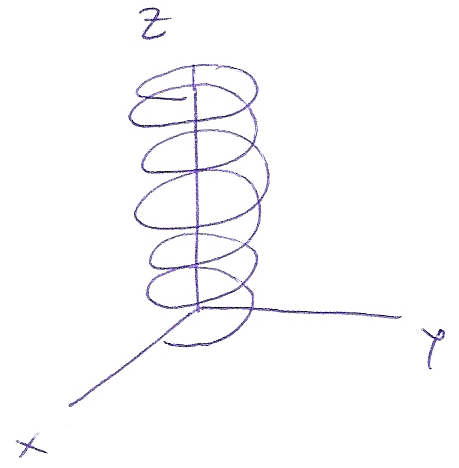
\includegraphics[width=6cm]{4.png}
				\caption{Looking at the origin from the z-axis, the helix traces out an ascending circular path starting at (1,0,0) and turning counterclockwise as $t$ increases.} \label{im:4}		
				\end{figure}\\				
	The helix can be generalized for radius $r$ and turn density $\frac{L}{n}$ as follows:
		\begin{flalign*} 
			&\text{\spaces1. }s(t) = \left(r\cos(t),r\sin(t),\frac{L}{2\pi n}t\right)&\\
			&\text{Thus it follows that}&\\
			&\text{\spaces2. }\diff s(t) = \left(-r\sin(t),r\cos(t),\frac{L}{2\pi n}\right) &\\
			&\text{\spaces3. }t_i = 0&\\
			&\text{\spaces4. }t_f = 2\pi n&
		\end{flalign*}	
	Okay, now what if we want a solenoid pointing in an arbitrary direction? For the unmodified equation, the helix circles upwards in the +z direction. So let's define the default helix direction vector $\hat{a}$ to be $(0,0,1)$. If we want the solenoid to be pointing in the arbitrary direction $\hat{b}$, then we want to find a rotation matrix $\mathbf{R}$ that rotates $\hat{a}$ onto $\hat{b}$ (Figure 2).
			\begin{figure}[ht!] 
				\centering
				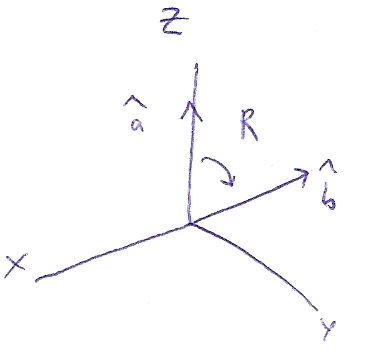
\includegraphics[width=5cm]{5.png}
				\caption{A rotation matrix $\mathbf{R}$ would rotate $\hat{a}$ onto $\hat{b}$. The rotated helix would circle counterclockwise along the $\hat{b}$ axis.} \label{im:5}		
				\end{figure}
				
	Turning to the internet, the source http://math.stackexchange.com/questions/180418/calculate-rotation-matrix-to-align-vector-a-to-vector-b-in-3d/476311 answers this question. The following is copied verbatim:
	
	Suppose you want to find a rotation matrix $\mathbf{R}$ that rotates unit vector $\hat{a}$ onto unit vector $\hat{b}$. Proceed as follows:

	Let $\vec{v} = \hat{a} \times \hat{b}$

	Let $s = \|v\|$ (sine of angle)

	Let $c = \hat{a} \cdot \hat{b}$ (cosine of angle)

	Then the rotation matrix R is given by:
		$$\mathbf{R} = \mathbf{I} + [\vec{v}]_{\times} + [\vec{v}]_{\times}^2{1-c \over s^2},$$

	where $[\vec{v}]_{\times}$ is the skew-symmetric cross-product matrix of $v$,
	$$[\vec{v}]_{\times} \stackrel{\rm def}{=} \begin{bmatrix}
		\,\,0 & \!-v_3 & \,\,\,v_2\\
		\,\,\,v_3 & 0 & \!-v_1\\
		\!-v_2 & \,\,v_1 &\,\,0
	\end{bmatrix}.$$
	
	End verbatim. Also, $\mathbf{I}$ is the identity matrix.

	This process fails with only two cases: If $\hat{a}$ is parallel with $\hat{b}$ and if $\hat{a}$ is antiparallel with $\hat{b}$. Thus, to account for these two cases, do the following: \\
	\spaces 1. If $s = 0$,\\
	\spaces\spaces a. If $c > 0$, set $\mathbf{R}$ to $\mathbf{I}$.\\
	\spaces\spaces b. If $c < 0$, set $\mathbf{R}$ to $-\mathbf{I}$.\\
	\spaces\spaces c. If $c = 0$, set $\mathbf{R}$ to $\mathbf{0}$.
	
	Since this $\mathbf{R}$ is constant for any given solenoid, we only need to compute the value of $\mathbf{R}$ once when initializing the solenoid. Afterwards, we just reference it from memory. Furthermore, because rotation is a linear transformation, this does not make finding the derivative any more complicated so yay. Our rotated solenoid would circle counterclockwise if we look at the origin from $\hat{b}$, travelling up along $\hat{b}$ (Figure 3).
		\begin{figure}[ht!] 
				\centering
				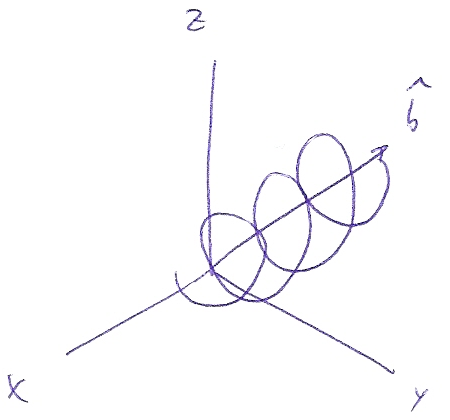
\includegraphics[width=5cm]{6.png}
				\caption{A rotated solenoid circling up along a $\hat{b}$ axis.} \label{im:6}		
				\end{figure}	\\
	Thus, for a solenoid rotated away from the default helix by rotation matrix $\mathbf{R}$:	
	\begin{flalign*} 
			&\text{\spaces1. }s(t) = \mathbf{R}
				\begin{bmatrix}
					r\cos(t) \\
					r\sin(t) \\
					\frac{L}{2\pi n}t
				\end{bmatrix} \\
			&\text{\spaces2. }\diff s(t) = \mathbf{R}
				\begin{bmatrix}
					-r\sin(t) \\
					r\cos(t) \\
					\frac{L}{2\pi n}
				\end{bmatrix} \\
			&\text{\spaces3. }t_i = 0&\\
			&\text{\spaces4. }t_f = 2\pi n&
		\end{flalign*}	
	The only modification is that we have left multiplied the equations in 1 and 2 by the rotation matrix~$\mathbf{R}$. So now that we have $s(t)$ and $\diff s(t)$, we can use the Runge-Kutta algorithm of choice to integrate from $t_i$ to $t_f$ for each wire and sum the results of each wire to get the net $\vec{B}$ at point $\vec{P}$.
	
	\subsubsection*{Choosing a time interval}
	
	We want to ensure that our integration covers the entirety of the length of the wire and doesn't end prematurely because the chosen $dt$ doesn't divide wholly into $t_f - t_i$. Thus, the program chooses a custom time interval $h$ depending on the wire:
			$$ h = \cfrac{t_f - t_i}{\left \lfloor \cfrac{t_f - t_i}{dt}\right \rceil}$$
	Where $\lfloor \rceil$ denotes the nearest integer function and $dt$ denotes the time interval chosen by the user. The above formula gives the time interval closest in value to the chosen $dt$ that divides wholly into the wire parameterization. This improves accuracy.
	
	\subsubsection*{TODO:}
	
	How to determine the accuracy for a given RK algorithm and d$t$ interval? \\
	\spaces -Simulate a solved system, e.g. a length of wire or a circle of wire; compare residuals of different sim settings \\
	\spaces -Compare simulated values with measured values in real life; compare residuals of different sim settings \\
	\spaces 
	
	

\end{document}